\section{Investigación previa}

\subsection{Datos en linux hardware}

Cuando se decide instalar Linux en una laptop, el primer paso crucial es verificar la compatibilidad del hardware con el sistema operativo. No todas las distribuciones funcionan de manera óptima en todos los equipos, ya que algunos pueden presentar problemas con los \textit{drivers}, rendimiento o compatibilidad con componentes específicos, como tarjetas gráficas dedicadas, conectividad Wi-Fi y funciones de suspensión.
\\\\
Por esta razón, lo primero que hice fue buscar mi laptop en \href{https://linux-hardware.org/}{Linux Hardware}, una base de datos comunitaria donde los usuarios reportan su experiencia con distintas distribuciones en diversos modelos de computadoras. Esta investigación me permitió evaluar qué tan bien funcionaba mi equipo con Linux y anticipar posibles inconvenientes.
\\\\
Tras analizar varias opciones, descubrí que la mejor distribución para mi laptop era \textbf{Pop! OS}, ya que está optimizada para hardware moderno y cuenta con soporte nativo para tarjetas gráficas NVIDIA y AMD. Además, su enfoque en la productividad y facilidad de uso la convierten en una opción ideal para desarrolladores y usuarios avanzados.
\\\\
Pop! OS destaca como la mejor opción para la \textbf{Asus TUF Gaming A15} debido a su optimización para hardware de alto rendimiento y su excelente compatibilidad con tarjetas gráficas dedicadas, como las NVIDIA que equipa este modelo. Esta distribución, desarrollada por System76, ofrece una versión con controladores propietarios preinstalados, lo que garantiza un mejor desempeño en juegos, aplicaciones de desarrollo y tareas exigentes. Además, su enfoque en la productividad y su integración con herramientas avanzadas de administración de GPU hacen que sea una opción ideal para usuarios que buscan un equilibrio entre rendimiento y facilidad de uso. Si bien existen otras distribuciones optimizadas para gaming, como Fedora o Nobara, Pop! OS destaca por su estabilidad, actualizaciones constantes y su capacidad para gestionar de manera eficiente la energía en laptops gaming, maximizando la autonomía sin sacrificar potencia.
\\\\
\begin{figure}[h]
  \centering
  \label{fig:img_linux_hardware}
  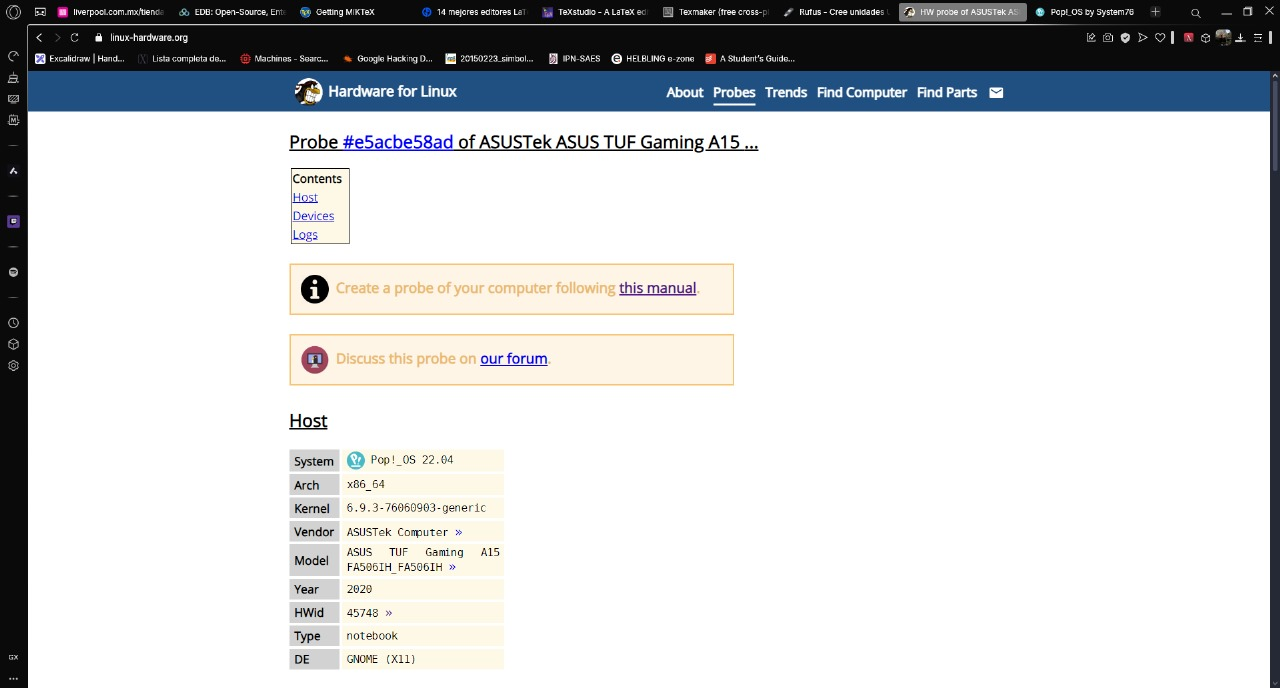
\includegraphics[width=0.95\textwidth]{./img/revision_linux-hardware.jpeg}
  \caption{Prueba en linux hardware}
\end{figure}

\clearpage

\subsection{Requerimientos de Pop OS}

\subsubsection{Requerimientos minimos}

\begin{itemize}
  \item \textbf{Procesador:} CPU de 64 bits
  \item \textbf{RAM:} 4GB
  \item \textbf{Almacenamiento:} 20GB
\end{itemize}

\\\\
Los requerimentos recomendados son de una RAM de 8GB y todo lo demas igual.
